\documentclass[12pt,a4paper,oneside]{book} 

%%%%%%%%%%%%%%%%%%%%%%%%%%%%%%%%%%%%%%%%%%%%%%%%%%%%%%%%%%%%%%%%%%%%%%%%
\usepackage{comment}
\usepackage{physics}
\usepackage[table,xcdraw]{xcolor}
\usepackage{ifthen}
\usepackage{graphicx}
\usepackage[dvips]{epsfig}
\usepackage{enumerate}
\usepackage{calc}
\usepackage{multicol} 
\usepackage{titlesec}
%\usepackage{showkeys}

%%%%%%%%%%%%%%%%%%%%%%%%%%%%%%%%%%%%%%%%%%%%%%%%%%%%%%%%%%%%%%%%%%%%%%%%

\usepackage{a4}
\usepackage{amsfonts}
\usepackage{amssymb}
\usepackage{epsfig}

%%%%%%%%%%%%%%%%%%%%%%%%%%%%%%%%%%%%%%%%%%%%%%%%%%%%%%%%%%%%%%%%%%%%%%%%

\usepackage{t1enc,times}
\usepackage{latexsym,amssymb}
\usepackage{amsmath}
\usepackage{amstext}
%\usepackage[T1]{fontenc}
%\usepackage{cmbright}
\usepackage{pifont}
\usepackage{marvosym}
%\usepackage{pslatex}
\usepackage{stmaryrd}
%\usepackage{txfonts}  

%%%%%%%%%%%%%%%%%%%%%%%%%%%%%%%%%%%%%%%%%%%%%%%%%%%%%%%%%%%%%%%%%%%%%%%%%%%%%%%

\usepackage{fancybox} 
\usepackage{fancyhdr}
\usepackage{fullpage}

%%%%%%%%%%%%%%%%%%%%%%%%%%%%%%%%%%%%%%%%%%%%%%%%%%%%%%%%%%%%%%%%%%%%%%%%%%%%%%%

%\usepackage{url}    
%\ExecuteOptions{dvips}
%\usepackage[pdftex,colorlinks=true]{hyperref}
%\hypersetup{backref,pdfpagemode=UseThumbs,pdfstartview=Fit,
%pdfpagelayout=SinglePage,pdfstartpage=1,colorlinks=true,menucolor=msc,
%anchorcolor=msc,pagecolor=msc,urlcolor=rfr,breaklinks=true,hyperfootnotes=true}

%%%%%%%%%%%%%%%%%%%%%%%%%%%%%%%%%%%%%%%%%%%%%%%%%%%%%%%%%%%%%%%%%%%%%%%%%%%%%%%

\pagestyle{plain}
\fancyhf{} 
%\renewcommand{\headrulewidth}{1pt}
%\renewcommand{\footrulewidth}{1pt}
\renewcommand{\headwidth}{\textwidth}
\fancyhead[LE]{\leftmark}
\fancyhead[RO]{\small \rightmark}
\fancyfoot[C]{\thepage}

%%%%%%%%%%%%%%%%%%%%%%%%%%%%%%%%%%%%%%%%%%%%%%%%%%%%%%%%%%%%%%%%%%%%%%%%%%%%%%%

\tolerance 4000
\textwidth 17.00cm
\topmargin -0.30cm
\oddsidemargin -0.25cm
\evensidemargin -0.25cm
\textheight 23.00cm
%\headsep 12pt
\headheight 15pt
\footskip 60pt
%\parindent 12pt

%%%%%%%%%%%%%%%%%%%%%%%%%%%%%%%%%%%%%%%%%%%%%%%%%%%%%%%%%%%%%%%%%%%%%%%%%%%%%%%

\renewcommand{\rmdefault}{ptm}  % times
\renewcommand{\rmdefault}{phv}  % helvetica
\renewcommand{\rmdefault}{pbk}  % bookman
\renewcommand{\rmdefault}{ppl}  % palatino
\renewcommand{\sfdefault}{phv}  % helvetica as sans serif
\renewcommand{\ttdefault}{pcr}  % courier as fixed width
\renewcommand{\tabcolsep}{8pt}
\renewcommand{\arraystretch}{1.25}

%%%%%%%%%%%%%%%%%%%%%%%%%%%%%%%%%%%%%%%%%%%%%%%%%%%%%%%%%%%%%%%%%%%%%%%%%%%%%%%

\def\nn{\nonumber}
\def\f{{\frac}}
\def\pa{{\partial}}
\def\d{{\rm d}}
\def\l{\left}
\def\r{\right}
\def\Mpl{M_{_{\rm Pl}}}

%%%%%%%%%%%%%%%%%%%%%%%%%%%%%%%%%%%%%%%%%%%%%%%%%%%%%%%%%%%%%%%%%%%%%%%%%%%%%%%

\def\done{\marginpar {\scriptsize DONE}}
\def\check{\marginpar {\scriptsize CHECK}}

%%%%%%%%%%%%%%%%%%%%%%%%%%%%%%%%%%%%%%%%%%%%%%%%%%%%%%%%%%%%%%%%%%%%%%%%%%%%%%%

\begin{document}

%%%%%%%%%%%%%%%%%%%%%%%%%%%%%%%%%%%%%%%%%%%%%%%%%%%%%%%%%%%%%%%%%%%%%%%%%%%%%%%

\baselineskip 20pt

%%%%%%%%%%%%%%%%%%%%%%%%%%%%%%%%%%%%%%%%%%%%%%%%%%%%%%%%%%%%%%%%%%%%%%%%%%%%%%%

\pagenumbering{roman}

%%%%%%%%%%%%%%%%%%%%%%%%%%%%%%%%%%%%%%%%%%%%%%%%%%%%%%%%%%%%%%%%%%%%%%%%%%%%%%%

\thispagestyle{empty}
\topskip 15pt
\hrule\hrule\hrule\hrule\hrule
\vskip 20pt
\centerline{\Huge \bf A polarimetric method for predicting } 
\vskip 15pt
\centerline{\Huge \bf  the Gravitational Wave polarizations} 
\vskip 15pt
\centerline{\Huge \bf of LISA Verification Binaries} 
\vskip 20pt
\hrule\hrule\hrule\hrule\hrule
\vskip 30pt
\centerline{\Large A project report}
\vskip 8pt
\centerline{\Large by}
\vskip 8pt
\centerline{\Large \bf Pranav Satheesh}
\vskip 8pt
\centerline{\Large Indian Institute of Technology Madras}
\vskip 140pt
\centerline{\Large Under the supervision of}
\vskip 10pt
\centerline{\Large  Prof. Prasenjit Saha}
\vskip 10pt
\centerline{\Large  University of Zurich}
%%%%%%%%%%%%%%%%%%%%%%%%%%%%%%%%%%%%%%%%%%%%%%%%%%%%%%%%%%%%%%%%%%%%%%%%%%%%%%%


\newpage\topskip 40pt
\centerline{\Large CERTIFICATE}
\thispagestyle{empty}
\vskip 20pt\noindent 
This is to certify that the project titled {\bf } is a bona fide record of work done by 
{\bf Pranav Satheesh} towards the fulfillment of credit  
requirements for summer project as part of the Dual Degree curriculum.
\vskip 120pt
\hspace{240pt}(Prasenjit Saha, Project supervisor)

%%%%%%%%%%%%%%%%%%%%%%%%%%%%%%%%%%%%%%%%%%%%%%%%%%%%%%%%%%%%%%%%%%%%%%%%%%%%%%%



%%%%%%%%%%%%%%%%%%%%%%%%%%%%%%%%%%%%%%%%%%%%%%%%%%%%%%%%%%%%%%%%%%%%%%%%%%%%%%%

\newpage\topskip 40pt
\thispagestyle{empty}
\centerline{\Large ABSTRACT}
\vskip 20pt\noindent 
Verification binaries are compact Galactic binaries with orbital periods of a few hours are gravitational wave sources in the mHz regime that
are expected to be detected by the Laser Interferometer Space Antenna
(LISA) and other future GW detectors. Binary system parameters such
as the inclination, orientation and distance are needed to provide an accu-
rate prediction of the gravitational wave strain. A full gravitational wave
polarisation prediction requires resolving the orientation of the binary or-
bit in the sky. We suggest that spectropolarimetry could be used to detect
the polarized light originating at the brighter star but scattered off the
fainter star, and hence measure the orientation of a verification binary. A
good candidate is the cataclysmic variable (AM CVn) HP Lib.
%%%%%%%%%%%%%%%%%%%%%%%%%%%%%%%%%%%%%%%%%%%%%%%%%%%%%%%%%%%%%%%%%%%%%%%%%%%%%%%

\newpage
\thispagestyle{empty}
%\tableofcontents
\newpage

%%%%%%%%%%%%%%%%%%%%%%%%%%%%%%%%%%%%%%%%%%%%%%%%%%%%%%%%%%%%%%%%%%%%%%%%%%%%%%%

\pagenumbering{arabic}

%%%%%%%%%%%%%%%%%%%%%%%%%%%%%%%%%%%%%%%%%%%%%%%%%%%%%%%%%%%%%%%%%%%%%%%%%%%%%%%

\section*{Introduction}

 Gravitational Wave polarization for verification binaries can be detected if the orientation and inclination are measured. Thus it is essential to measure them from electromagnetic radiation.


\section*{Gravitational Waves}

\subsection*{Linearized Einstein Equations}

Gravitational Waves emerge from Enistein's theory of General Relativity. In the "linearized theory" we can expand the Einstein equations around the flat Minkowski metric $\eta_{\mu \nu}$. It is easy to realise that the quations gets simplified into a wave equation and can be further written in a simple form by suitable gauge choice.

The Einstein equations,

\begin{equation}
\label{eq:Einstein-eq}
R_{\mu \nu} - \frac{1}{2} g_{\mu \nu} R = \frac{8 \pi G}{c^4} T_{\mu \nu}
\end{equation}

are expanded around the flat spacetime metric

\begin{equation}
\label{lingmunu}
g_{\mu \nu} = \eta_{\mu \nu} + h_{\mu \nu}, \qquad |h_{\mu \nu}| << 1
\end{equation}

Where $R_{\mu \nu}$ is the Ricci tensor, $R$ is the Ricci scalar and $T_{\mu \nu}$ is the energy-momentum tensor. In the \textit{linearized theory}, the equations of motions are all expanded to linear order in $h_{\mu \nu}$.The linearised equation in the so-called \emph{Lorentz gauge} ($\partial^{\nu} \bar{h}_{\mu \nu} = 0$) becomes

\begin{equation}
\label{eq:Wave-eq-Lorenz}
\Box \bar{h}_{\mu \nu} = - \frac{16 \pi G}{c^4} T_{\mu \nu}
\end{equation}

Where
\begin{equation}
\label{eq: hbar}
\bar{h}_{\mu \nu} = h_{\mu \nu} - \frac{1}{2} \eta_{\mu \nu}
\end{equation}

This is a wave equation where $\Box$ represents the d'Alembertian operator $\Box = - (1/c^2)\partial^2_{t} + \nabla^2$. Outside the source, $T_{\mu \nu} = 0$. 

\begin{equation}
\label{eq:Wave-eq-Outside}
\Box \bar{h}_{\mu \nu} = 0
\end{equation}

The Lorenz gauge reduced the 10 degrees of freedom of the symmetric matrix $h_{\mu \nu}$ to six. We can further do a coordinate transformation $x^{\mu} \rightarrow x^{\mu} + \xi^{\mu}$ where the $\xi$ function satisfies

\begin{equation}
\label{eq:xi}
\Box \xi_{\mu} = 0
\end{equation}

One can show we can choose $\xi^{\mu}$ to impose four conditions on $h^{\mu \nu}$. This further reduces the degrees of freedom from six to two. We thus have the \emph{transverse-traceless gauge} (or TT-gauge) defined by

\begin{equation}
\label{eq: TT gauge}
h^{0 \mu} = 0, \quad h^{i}_{i} = 0, \quad \partial^{j}h_{ij} = 0
\end{equation}
The TT-Gauge will be denoted by $h^{TT}_{ij}$.


\subsection*{Gravitational Wave Polarizations}

 We can now write plane wave solutions to the equation \eqref{eq:Wave-eq-Outside}. Choosing the propogation axis along the z axis we find that in the TT gauge
 
\begin{equation}
\label{eq:Wave-eq-sol}
h^{TT}_{ij}(t,z) = \begin{pmatrix}
0 & 0 & 0 & 0 \\
0  & h_{+} & h_{\cross} & 0 \\
0 & h_{\cross} & -h_{+} & 0 \\
0 & 0 & 0 & 0
\end{pmatrix}_{ij} \ \cos[\omega (t - z/c)]
\end{equation}

or

\begin{equation}
\label{eq:Wave-eq-sol-pol}
h^{TT}_{ab}(t,z) = \begin{pmatrix}
h_{+} & h_{\cross} \\
h_{\cross} & -h_{+}  \\
\end{pmatrix}_{ab} \ \cos[\omega (t - z/c)]
\end{equation}

where the indices $a,b = 1,2$ indicates the two  polarizations of the wave. These are called \emph{plus} and \emph{cross} polarizations. We can visualise the two polarization modes on the deformation of a ring of test masses caused by the gravitational waves.


\begin{figure}[!hb]
\centering
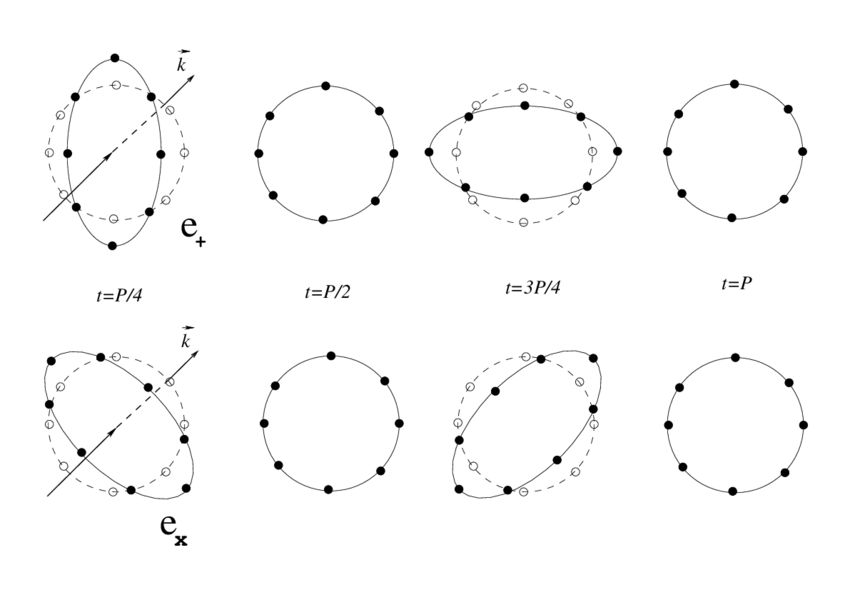
\includegraphics[scale=0.45]{../Figures/Schematic-deformations-produced-on-a-ring-of-freely-falling-particles-by-gravitational.png}
\caption{The two polarization modes}
\label{fig:polarization-viz}
\end{figure}
 

\subsection*{Gravitational Waves from inspiralling compact binaries}

Most important and significant sources of GWs are from binary compact objects, neutron stars and black holes. We can show that the GW amplitude in the TT-gauge can be described using the Mass quadrupole radiation formulae

\begin{equation}
\label{eq: Quadrupole formula}
h^{TT}_{ij} = \frac{1}{r} \frac{2 G}{c^4} \ddot{Q}_{ij}^{TT}(t-r/c)
\end{equation}

where the quadrupole moment is defined by 

\begin{align}
Q^{ij} &= M^{ij} - \frac{1}{3} \delta^{ij} M_{kk} \\
       &= \int d^3 x \, \rho(t,\textbf{x}) (x^i x^j - \frac{1}{3} r^2 \delta^{ij})
\end{align}

Note that $M^{ij}$ is the momenta of the energy density $T^{00} (\rho c^2)$ defined as

\begin{equation}
M^{ij} = \frac{1}{c^2} \int d^3 x  \, T^{00}(t,\textbf{x}) \, x^i x^j 
\end{equation}

It is then straightforward to show that the two polarization amplitudes for a GW propogating in the z direction is given by

\begin{align}
\label{eq:hphcfromquad}
h_{+} &= \frac{G}{c^4 \ r} (\ddot{M}_{11} - \ddot{M}_{22})\\
h_{\cross} &= \frac{2 \ G}{c^4 \ r} \ddot{M}_{12}
\end{align}

For the cass of two inspiralling compact binaries of masses $m_1$ and $m_2$ at a seperation of $R$, we can show that \eqref{eq:hphcfromquad} becomes

\begin{align}
\label{eq:hphcfrombinary}
h_{+} &= \frac{4 G \mu \omega^2 R^2}{c^4 \ r} \Bigl(\frac{1 + cos^2 \iota}{2}\Bigr) \cos(2 \phi) \\
h_{\cross} &= \frac{4 G \mu \omega^2 R^2}{c^4 \ r} (cos \, \iota) \sin(2 \phi)
\end{align}

where the angle $\iota$ is the inclination angle of the orbit and $\phi$ is the angle swept along the orbital plane.


\section*{LISA and Binary Configuration}

The ground based detectors have so far detected over 20 binary black holes, binary neutron star and a neutron star-black hole collisions so far. They operate above 10 Hz frequency as shown in the sensitivity curve. LISA on the other hand will operate in the mHz region which is potentially rich in GW sources. LISA consists of three spacecrafts seperated by about 5 million kms in an equilateral triangle configuration. LISA will orbit around the sun and the center of the triangle will be kept at a distance about 50 million kms behind the Earth. 


\subsection*{Coordinate System}

For our calculations, the coordinate system as described by the figure is what we will follow. For the sake of simplicity, we just consider one of the arm of LISA and and align the z-axis with the line of sight direction from the center of mass of the binary. The angular momentum of the binary is inclined by an angle $\iota$. This is the angle of inclination. We take the arm to be in the x-z plane and at angle $\phi$ with respect to the line of sight. The binary has a position angle $\Psi$ which applies a rotation to $h_{+}$ and $h_{×}$ and is the polarization angle. We will show that, to give an accurate prediction of the the polarizations, one needs to calculate the orientation ($\iota$,$\Psi$) with a sufficient accuracy.

\begin{figure}[!htb]
\centering
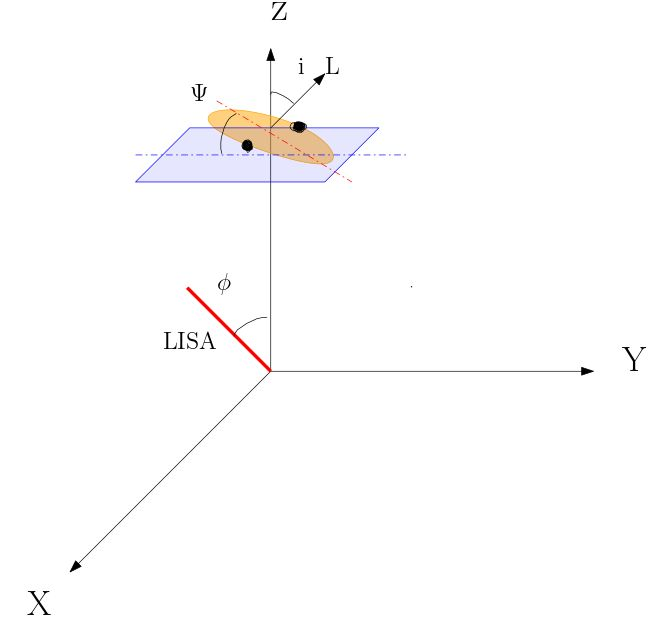
\includegraphics[scale=0.5]{../LISA_orientation1.jpg} 
\caption{Details about the coordinate system}
\end{figure}

\subsection*{Detector Response}

The strain measured by a detectior is written as 
\begin{equation}
\label{eq:detector_strain}
h = h_{+} F_{+} + h_{\cross} F_{\cross}
\end{equation}
where $F_{+}$ and $F_{\cross}$ are \emph{antenna pattern factors}. The pattern functions depend on the orientation of the detector.
For LISA the pattern functions can be found at.
 
The measurement of the strain is not instantaneous as it takes a finite aount of time $t = L/c$ , where $L$ is the length of the arm. It is thus required to integrate the strain along the photon's path.

\begin{align}
\label{eq: photon path}
\frac{c}{L} \int_{t - L/c}^{t} h_{+}(t^{'}) dt^{'} &= \frac{\Delta L_{+}(t)}{L} \\
\frac{c}{L} \int_{t - L/c}^{t} h_{\cross}(t^{'}) dt^{'} &= \frac{\Delta L_{\cross}(t)}{L}
\end{align}

\section*{Verification Binaries}

The future LISA mission will cover low-frequency gravutational  wave detections and thus potentially detect signals from Galactic Binaries. LISA guarantees the detection of GW's from stellar mass binary systems that are strong enough to be detected and studied through electromagnetic observations. They will be crucial in testing the proper functionality of LISA. The detection of GWs from these systems will also open up the door to study the physics of compact objects. The verification binaries comprise of 

\begin{itemize}
\item AM CVn Binary Systems
\item Double White Dwarf Binaries
\item Ultra- compact X-ray binaries
\item Cataclysmic Variables (CV)
\end{itemize}

Some of these binaries are being expected to be detected on a timescale of weeks or a few months (cite Stroer and Vecchio 2006). The GW strain depends on the masses of the binary components, orientation of the orbit and their distance. Masses can be calculated from orbital spectroscopy, combined with Roche-lobe Geometry. Orbital inclination, however is poorly constrained. Hence, we need to look at alternate methods of measuring orbital orientation like using polarimetry. The table adapted from shows a sample of measured physical properties of verification binaries. 


% Please add the following required packages to your document preamble:
% \usepackage[table,xcdraw]{xcolor}
% If you use beamer only pass "xcolor=table" option, i.e. \documentclass[xcolor=table]{beamer}
\begin{table}[!htb]
\centering
\begin{tabular}{|l|l|l|l|l|}
\hline
Source                                 & Orbital Period (sec)                    & $m_1$ ($M_{\odot})$                       & $m_2$ ($M_{\odot})$                         & $\iota$ (deg)                         \\ \hline
HM Cnc                                 & 321.529                                 & 0.55                                      & 0.27                                        & $\approx$ 38             \\ \hline
AM CVn                                 & 1028.73                                 & 0.68 $\pm$ 0.06              & 0.125
$\pm$ 0.012              & 43 $\pm$ 2                 \\ \hline
{\color[HTML]{FE0000} \textbf{HP Lib}} & {\color[HTML]{FE0000} \textbf{1102.70}} & {\color[HTML]{FE0000} \textbf{0.49-0.80}} & {\color[HTML]{FE0000} \textbf{0.048-0.088}} & {\color[HTML]{FE0000} \textbf{26-34}} \\ \hline
CR Boo                                 & 1471.3                                  & 0.67-1.10                                 & 0.044-0.088                                 & 30                                    \\ \hline
V803 Cen                               & 1596.4                                  & 0.78-1.17                                 & 0.059-0.109                                 & 12-15                                 \\ \hline
\end{tabular}
\caption{Physical porperties of Verification Binaries}
\end{table}








\section*{Target Source: HP Lib}

AM CVn stars are helium-rich consisting of a low mass donor star and a high mass accretor star, with a binary orbital periods are less than 65 minutes. The binary system evolve through a common envelope (CE) channel. HP Lib consists of a high-mass white dwarf and a low-mass star, a brown dwarf. The masses of the binaries are measured from the lightcurves.cite  also gives the masses $M_{1}$ and $M_{2}$ and the inclination of the system is reported in cite.

Also, the radius of the secondary can be found using the reation mentioned in citep{Patterson}

\begin{equation}
R_{zs} = 0.0155 \ m_2^{-0.212}
\end{equation}
For $m_2 = 0.048$, $R_2 = 0.030$ in solar units.

\begin{table}[!htb]
\centering
\begin{tabular}{|c|c|c|c|c|}
\hline 
\rule[-1ex]{0pt}{2.5ex} Source & $m_1$($M_{\odot}$) & $m_2$($M_{\odot}$) & $P_{\rm orb}$(sec) &i (degrees) \\ 
\hline 
\rule[-1ex]{0pt}{2.5ex} HP Lib & 0.49--0.80 & 0.048--0.08 & 1102.70 & 26-34\\ 
\hline 
\end{tabular}
\caption{The estimated values of mass and time period of HP Lib}
\label{table1}
\end{table}


\subsection*{Strain Calculations}

We can calculate the characteristic strain of the verification binaries to show that they fall withing the sensitivity of LISA. The gravitational wave ampltude is given by


\begin{equation}
\label{eq:Amplitude}
\mathcal{A} = \frac{2 (G \mathcal{M})^{5/3}}{c^4 d} (\pi f)^{2/3}
\end{equation}
where $\mathcal{M}$ is the chirp mass, $\mathcal{M} = (m_1 m_2)^{3/5}/(m_1 + m_2)^{1/5}$, $d$ is the distance to the source and $f$ is the gravitational wave frequency $f = 2/P_{orb}$. The characteristic strain ($h_c$) is calculated as 

\begin{equation}
\label{eq:hc}
h_{c} = \sqrt{N_{cycle}} \mathcal{A}
\end{equation}

where $N_{cycle} = fT_{obs}$. LISA will observe for a period of four years. The characteristic strain is calculated for 13 disystems that have an SNR$\geq 5$. The SNR is calculated after 4 years of integration wuth LISA.

\begin{figure}[!htb]
\centering
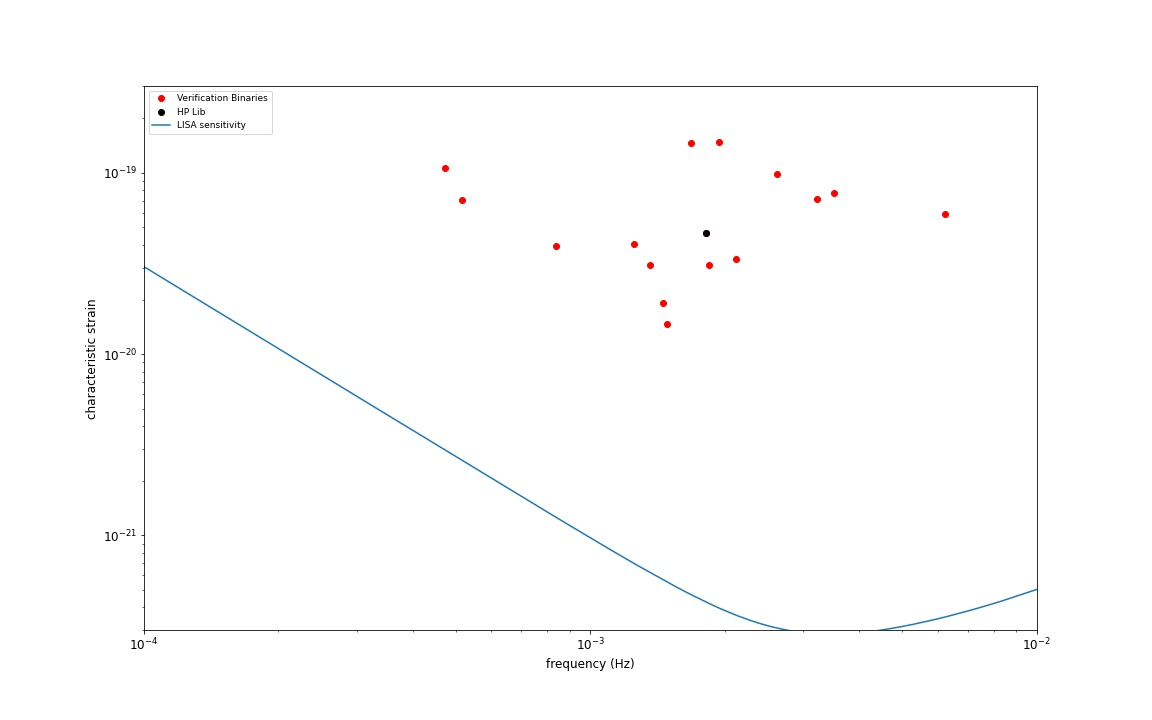
\includegraphics[scale=0.3]{../strain_verific_binary.jpg} 
\caption{Verification binaries}
\end{figure}

From eq 19-20 we find the polarization prediction to be
\begin{align}
\frac{\Delta L_{+}}{L} &= \frac{G \mu R^2 \omega \cos(2 \Psi) \cos(\phi) (3 + \cos(2 \iota)) \sin(\frac{L \omega}{c}))}{c^3 \, r \, L}\\
\frac{\Delta L_{\cross}}{L} &= \frac{4 G \mu R^2 \omega \cos(2 \Psi) \cos(\phi) \cos(\iota) \sin(\frac{L \omega}{c}))}{c^3 \, r \, L}\\
\end{align}
The length of LISA arm $L = 2.5 \cross 10^9 m$. We can now estimate the error involved in the polarization amplitude for HP-Lib. The figure shows the error in estimation of the polarization amplitudes as a function of the orientation of the binary $\Psi$.

\begin{figure}[!htb]
\centering
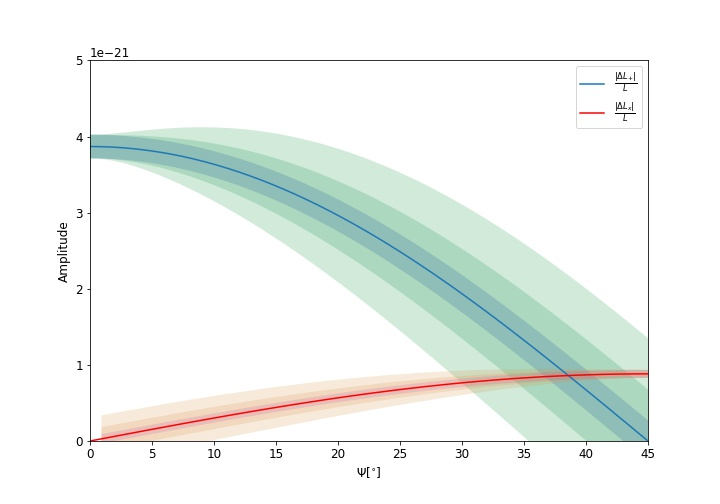
\includegraphics[scale=0.6]{../LISA_ampitude_variation.jpg} 
\caption{Amplitudes}
\end{figure}

\section*{Polarimetric Method}

Measuring polarization angles as a function of orbital phase can in principle be used to determine the orbit of a binary. In a polarimetric orbit is constructed from polarimetric observations. Such work was done previously on symbiotic stars. This is done by fitting the parameters of the time period $P$, the time of phase conjunction $T_{0}$, the orientation (line of nodes) of the orbital plane $\Omega$ anf the orbital inclination $i$. 

We propose a similar method on the estimation of the orientation and the inclination angle for verification binaries. We aim to study the system HP-Lib using \textbf{ALFOSC} (Alhambra Faint Object Spectrogtaph and Camera), at the Astronomical Observatory, Neils Bhor Institute of Astronomy.

HP~Lib is a cataclysmic variable consisting of a white dwarf of mass
$m_1=0.49\,$--$\,0.80\,M_\odot$ and a probable brown dwarf of mass
$m_2=0.048\,$--$\,0.08\,M_\odot$ in a orbit with period
$1102.70\rm\,s$ and inclination of $26^\circ$--$34^\circ$.  A
periodogram of the light curve includes the so-called superhump, a
wide distribution of frequencies around the orbital period of the
system, caused by the presence of a precessing accretion disc.\\

A faint but detectable polarisation signal is expected from light
reflected off the fainter companion, that will be modulated with the
orbital period. The detection and characterization of this signal
would allow the determination of the PA of the orbit, leading to a
prediction of the gravitational-wave polarisation (Fig.~1).  Note that there
is no intrinsic connection between optical and gravitational-wave
polarisation, that both appear here is serendipitous.

The fraction of scattered light can be estimated as follows.  First,
following Patterson et al.~(2002) we estimate the radius of the
secondary as
\begin{equation}
R_2 = 0.0155 \ m_2^{-0.212}
\end{equation}
For $m_2 = 0.048M_\odot$, $R_2 = 0.030R_\odot$.  Assuming the system
is degenerate, smaller masses correspond to larger radii.  Writing $L$
for the luminosity of the primary, the flux at a distance $d$ is given
by $L/4 \pi d^2$. The cross section area for brown dwarf is $\pi R_2^2$.
Therefore, the total flux received is:
\begin{equation}
\frac{L}{4 \pi d^2} \ \pi R^2 = \frac{L}{4} \ \left(\frac{R}{d}\right)^2
\end{equation}
From Kepler's third law, using the Earth's orbit as a reference, we have
\begin{equation}
  \frac{1}{4} \left(\frac{R_2}{\rm 1\,au}\right)^2
  \left(\frac{M}{M_{\odot}}\right)^{-2/3}
  \left(\frac{P}{P_{\oplus}}\right)^{-4/3}
\end{equation}

For a first estimate, we can take $R = 0.03R_\odot$ or $R/c \approx           
0.07$ which if we substitute above we estimate the fraction of light
received is $\approx 0.0064$. By monitoring HP Lib during one full 
night, we will be able to stack $\sim$25 periods and measure the
expected signal in polarization down to a fraction of a percent, that will help us 
constrain the orbital parameters. 


\section*{Concllusion}
HP Lib


\begin{thebibliography}{99}
%%%%%%%%%%%%%%%%%%%%%%%%%%%%%%%%%%%%%%%%%%%%%%%%%%%%%%%%%%%%%%%%%%%%%%%%%%%%%%%
% \bibitem{2df}
% See, {\tt http://magnum.anu.edu.au/~TDFgg/}.
% %%%%%%%%%%%%%%%%%%%%%%%%%%%%%%%%%%%%%%%%%%%%%%%%%%%%%%%%%%%%%%%%%%%%%%%%%%%%%%%
% \bibitem{sdss}
% See, {\tt http://www.sdss.org/}.
% %%%%%%%%%%%%%%%%%%%%%%%%%%%%%%%%%%%%%%%%%%%%%%%%%%%%%%%%%%%%%%%%%%%%%%%%%%%%%%%
% \bibitem{webb-1999}
% S.~Webb, {\sl Measuring the Universe}\/ (Springer, Berlin, 1999).
% %%%%%%%%%%%%%%%%%%%%%%%%%%%%%%%%%%%%%%%%%%%%%%%%%%%%%%%%%%%%%%%%%%%%%%%%%%%%%%%
% \bibitem{scp}
% See, {\tt http://supernova.lbl.gov/}.
% %%%%%%%%%%%%%%%%%%%%%%%%%%%%%%%%%%%%%%%%%%%%%%%%%%%%%%%%%%%%%%%%%%%%%%%%%%%%%%%
% \bibitem{snls}
% See, {\tt http://snls.in2p3.fr/}.
% %%%%%%%%%%%%%%%%%%%%%%%%%%%%%%%%%%%%%%%%%%%%%%%%%%%%%%%%%%%%%%%%%%%%%%%%%%%%%%%
% \bibitem{durrer-2008}
% R.~Durrer, {\sl The Cosmic Microwave Background}\/ (Cambridge University Press, 
% Cambridge, England, 2008).
% %%%%%%%%%%%%%%%%%%%%%%%%%%%%%%%%%%%%%%%%%%%%%%%%%%%%%%%%%%%%%%%%%%%%%%%%%%%%%%%
% \bibitem{padmanabhan-1999}
% T.~Padmanabhan, {\sl Theoretical Astrophysics, Volume III:~Galaxies and 
% Cosmology},\/ (Cambridge University Press, Cambridge, England, 1999).
%%%%%%%%%%%%%%%%%%%%%%%%%%%%%%%%%%%%%%%%%%%%%%%%%%%%%%%%%%%%%%%%%%%%%%%%%%%%%%%
\end{thebibliography}
%%%%%%%%%%%%%%%%%%%%%%%%%%%%%%%%%%%%%%%%%%%%%%%%%%%%%%%%%%%%%%%%%%%%%%%%%%%%%%%
\end{document}